\chapter{Alternating Polynomials} \label{ch:alternating-polynomials}

Consider the following two representations of \(\sym{n}\):
\begin{itemize}
    \item The trivial representation \(1 \colon \sym{n} \to \GL[1]{\complexes}\) given by \(\sigma \mapsto 1\).
    \item The sign representation \(\sign \colon \sym{n} \to \GL[1]{\complexes}\) given by \(\sigma \mapsto \sign(\sigma)\).
\end{itemize}

Consider any representation \(\phi \colon  \sym{n} \to \GL[1]{\complexes}\).
Let \(i \in \interval{n-1}\).
Then,
\begin{equation}
    \phi(\eltr{i}) = \phi(\tau \eltr{1} \tau^{-1}) = \phi(\tau) \phi(\eltr{1}) \phi(\tau)^{-1} = \phi(\eltr{1}),
\end{equation}
for some \(\tau \in \sym{n}\).
Thus, \(\phi(\eltr{i})\) is independent of \(i\).
Moreover, \(\phi(\eltr{i})^2 = \phi(\eltr{i}^2) = \phi(\id) = 1\), hence \(\phi(\eltr{i}) = \pm 1\), for all \(i \in \interval{n-1}\).
If \(\phi(\eltr{i}) = 1\) for all \(i \in \interval{n-1}\), then \(\phi = 1\).
If \(\phi(\eltr{i}) = -1\) for all \(i \in \interval{n-1}\), then \(\phi = \sign\).

Therefore, the only irreducible representations of \(\sym{n}\) of dimension \(1\) are the trivial representation and the sign representation.

Suppose \(\rho \colon \sym{n} \to \GL{V}\) is a representation of \(\sym{n}\).
The \vocab{invariants} of \(\rho\) are the elements \(v \in v\) such that
\begin{equation}
    \rho(w) v = 1(w) v, 
\end{equation}
for all \(w \in \sym{n}\), where \(1\) denotes the trivial representation.
We can alternatively call these elements \vocab{\(1\)-isotypic elements}.
Let \(\Inv(V)\) denote the set of \(1\)-isotypic elements of \(\rho \colon \sym{n} \to \GL{V}\).

We can replace the trivial representation with the sign representation.

The \vocab{\(\sign\)-isotypic elements} of \(\rho\) are the elements \(v \in V\) such that
\begin{equation}
    \rho(w) v = \sign(w) v,
\end{equation}
for all \(w \in \sym{n}\).
Let \(\Alt(V)\) denote the set of \(\sign\)-isotypic elements of \(\rho \colon \sym{n} \to \GL{V}\).

\begin{proposition}
    Let \(\rho \colon \sym{n} \to \GL{V}\) be a representation of \(\sym{n}\).
    Then, \(\Alt(V)\) is a subspace of \(V\).
\end{proposition}

\begin{definition}[Direct sum of representations]
    If \(\rho_1 \colon \sym{n} \to \GL{V_1}\) and \(\rho_2 \colon \sym{n} \to \GL{V_2}\) are representations of \(\sym{n}\),
    then the \vocab{direct sum} of \(\rho_1\) and \(\rho_2\) is the representation \(\rho_1 \oplus \rho_2 \colon \sym{n} \to \GL{V_1 \oplus V_2}\) given by
    \begin{equation}
        (\rho_1 \oplus \rho_2)(w) = \rho_1(w) \oplus \rho_2(w),
    \end{equation}
    for all \(w \in \sym{n}\).
\end{definition}

Much more interesting than adding two representations to get a third,
is to start with a representation and decompose it into a direct sum of other representations.

\begin{theorem}
    Let \(\rho \colon \sym{n} \to \GL{V}\) be a representation of \(\sym{n}\).
    Then, \(V = \Inv(V) \oplus \Alt(V) \oplus W\), for some \(W \subset V\),
    and 
    \begin{equation}
        \rho = 1_{\Inv(V)} \oplus \sign_{\Alt(V)} \oplus \rho|_W.
    \end{equation}
\end{theorem}

We saw that, if \(V\) is an algebra, then \(\Inv(V)\) is a subalgebra of \(V\).
However, this is not the case for \(\Alt(V)\).
Suppose \(a \in \Alt(V)\).
Then \(w \cdot a^2 = (w \cdot a) (w \cdot a) = \sign(w)^2 a^2 = a^2\), for all \(w \in \sym{n}\), which is not always equal to \(\sign(w) a^2\) (for \(n \geq 2\)).
Something can be salvaged from this situation.

\begin{theorem} \label{thm:inv-alt-subalgebra}
    Let \(V\) be an algebra.
    Let \(\rho \colon \sym{n} \to \Aut(V)\) be a representation of \(\sym{n}\).
    Consider the subspace \(\Inv(V) \oplus \Alt(V)\) of \(V\).
    Then, \(\Inv(V) \oplus \Alt(V)\) is a subalgebra of \(V\).
\end{theorem}

The proof of Theorem~\ref{thm:inv-alt-subalgebra} follows from Theorem~\ref{thm:inv-alt-super}.

\begin{definition}[\(G\)-graded algebra]
    A \vocab{\(G\)-graded algebra} is an algebra \(V\) together with a direct sum decomposition
    \begin{equation}
        V = \bigoplus_{g \in G} V_g,
    \end{equation}
    such that \(ab \in V_{gh}\), for all \(a \in V_g\) and \(b \in V_h\).
\end{definition}

A \vocab{superalgebra} is a \(\mathbb{Z}_2\)-graded algebra.

\begin{theorem} \label{thm:inv-alt-super}
    Let \(V\) be an algebra.
    Let \(\rho \colon \sym{n} \to \Aut(V)\) be a representation of \(\sym{n}\).
    Consider the subspace \(\Inv(V) \oplus \Alt(V)\) of \(V\).
    Then, \(\Inv(V) \oplus \Alt(V)\) is a superalgebra with parts \(\Inv(V)\) and \(\Alt(V)\).
\end{theorem}

\begin{proof}
    Let \(a \in \Inv(V)\) and \(b \in \Inv(V)\).
    Then, \(w \cdot (ab) = (w \cdot a) (w \cdot b) = a b\), for all \(w \in \sym{n}\).
    Thus, \(ab \in \Inv(V)\).
    Let \(a \in \Inv(V)\) and \(b \in \Alt(V)\).
    Then, \(w \cdot (ab) = (w \cdot a) (w \cdot b) = (\sign(w) a) b = \sign(w) a b\), for all \(w \in \sym{n}\).
    Thus, \(ab \in \Alt(V)\).
    Let \(a \in \Alt(V)\) and \(b \in \Alt(V)\).
    Then, \(w \cdot (ab) = (w \cdot a) (w \cdot b) = \sign(w)^2 a b = a b\), for all \(w \in \sym{n}\).
    Thus, \(ab \in \Inv(V)\).

    Therefore, \(\Inv(V) \oplus \Alt(V)\) is a subalgebra of \(V\),
    and \(\Inv(V) \oplus \Alt(V)\) is a superalgebra with parts \(\Inv(V)\) and \(\Alt(V)\).
\end{proof}

Now, apply this with \(\mathcal{A} = \rationals[x_1, x_2, \ldots, x_n]\),
and the action \(\rho \colon \sym{n} \to \Aut(\mathcal{A})\) given by
permuting the variables.
The \(\sign\)-isotypic elements of \(\mathcal{A}\) are are the \vocab{alternating polynomials},
denoted by \(\AltPoly(n)\) or \(v_n\Sym(n)\).

For example,
\begin{equation}
    x_1^2x_2 - x_2^2x_1 + x_2^2x_3 - x_3^2x_2 + x_3^2x_1 - x_1^2x_3 \in \AltPoly(3).
\end{equation}

\begin{lemma}
Let \(p \in \AltPoly(n)\).
Let \(\alpha\) be a composition of length \(n\).
Assume that \(\alpha_i = \alpha_j\) for some distinct \(i, j \in \interval{n}\).
Then, the coefficient of \(x^\alpha\) in \(p\) is zero.
\end{lemma}

\begin{proof}
    We compute that     
    \begin{equation}
        [x^\alpha] p = [x^alpha] (- \eltr{i, j} \cdot p) = - [x^\alpha] p,
    \end{equation}
    which implies that \([x^\alpha] p = 0\).
\end{proof}

\begin{definition}[Vandermonde polynomial]
    Define the \vocab{\(n\)\textsuperscript{th} Vandermonde polynomial} to be
    \begin{equation}
        v_n = \prod_{1 \leq i < j \leq n} (x_j - x_i) \in \AltPoly(n).
    \end{equation}
\end{definition}

\begin{lemma} \label{lem:vandermonde-divides-alt}
    Let \(p \in \AltPoly(n)\).
    Then, \(v_n \mid p\).
\end{lemma}

\begin{proof}
    Let \(i < j\) in \(\interval{n}\).
    If we specialize \(p\) by setting \(x_i = x_j\), then \(p \mapsto 0\).
    Therefore, \(x_i - x_j \mid p\).
    Since this holds for all \(i < j\), we have \(v_n \mid p\).
\end{proof}

\begin{lemma} \label{lem:vandermonde-times-sym-is-alt}
    Let \(p \in \AltPoly(n)\).
    Then, \(\frac{p}{v_n} \in \Sym(n)\).
\end{lemma}

\begin{proof}
    Let \(p \in \AltPoly(n)\).
    Then, \(p = v_n q\), for some \(q \in \rationals[x_1, x_2, \ldots, x_n]\),
    by Lemma~\ref{lem:vandermonde-divides-alt}.
    Since \(p, v_n \in \AltPoly(n)\),
    we have \(w \cdot p = \sign(w) p\) and \(w \cdot v_n = \sign(w) v_n\), for all \(w \in \sym{n}\).
    Thus, \(w \cdot q = q\), for all \(w \in \sym{n}\), and consequently, \(q \in \Sym(n)\).
\end{proof}

\begin{corollary}
    The map from \(\Sym(n)\) to \(\AltPoly(n)\) given by \(q \mapsto v_n q\) is a vector space isomorphism.
\end{corollary}

Note that bases of \(\Sym(n)\), multiplied by \(v_n\), form a basis of \(\AltPoly(n)\), and conversely, bases of \(\AltPoly(n)\), divided by \(v_n\), form a basis of \(\Sym(n)\).

Let's make one basis of \(\AltPoly(n)\) explicitly.

Given a partition \(\lambda\) of \(n\),
we define
\begin{equation}
    \tilde{a}_\lambda
    =
    \sum_{w \in \sym{n}}
    \sign(w)
    x^{w \cdot \lambda} \in \AltPoly(n).
\end{equation}
Note that, if \(\lambda\) has equal parts, then \(\tilde{a}_\lambda = 0\).
A \vocab{strict partition} is a partition with distinct parts.
The set 
\begin{equation}
    \{ \tilde{a}_\lambda \mid \lambda \text{ is a strict partition of } n \}
\end{equation}
is a basis of \(\AltPoly(n)\).

Let \(\delta_n = (n-1, n-2, \ldots, 1, 0)\).
Note that the map \(\lambda \mapsto \lambda + \delta_n\) is a bijection between strict partitions of \(n\) and partitions of \(n+1\).
Then, we define
\begin{equation}
    a_\lambda = \tilde{a}_{\lambda + \delta_n} \in \AltPoly(n+1),
\end{equation}
and consequently, 
\begin{equation}
    \{ a_\lambda \mid \lambda \in \Par(n) \}
\end{equation}
is a basis of \(\AltPoly(n+1)\).

If we have a basis of \(\AltPoly(n)\),
we can divide by \(v_n\) to get a basis of \(\Sym(n)\).

\begin{definition}[Schur polynomial]
    Let \(\lambda\) be a partition of \(n\).
    Define the \vocab{Schur polynomial} \(\schur{\lambda} \in \Sym(n)\) by
    \begin{equation}
        \schur{\lambda} = \frac{a_\lambda}{v_n} \in \Sym(n).
    \end{equation}
\end{definition}

\begin{proposition}[Jacobi's bialternant formula] \label{prop:jacobi-bialternant}
    Let \(\lambda\) be a partition of \(n\).
    Then,
    \begin{equation}
        \schur{\lambda} = 
        \frac{
            \det\left(\left[x_i^{\lambda_j + n - j}\right]\right)_{i, j \in \interval{n}}
        }{
            \det\left(\left[x_i^{n - j}\right]\right)_{i, j \in \interval{n}}
        }.
    \end{equation}
\end{proposition}

\begin{example}[\(n = 3\), \(\lambda  = \composition{2}\)]
    Let \(n = 3\).
    Then, \(\delta_3 = \composition{2, 1, 0}\)
    and
    \begin{equation}
        v_3 = a_{\composition{0, 0, 0}} = \tilde{a}_{\composition{2, 1, 0}} = x_1^2x_2 - x_2^2x_1 + x_2^2x_3 - x_3^2x_2 + x_3^2x_1 - x_1^2x_3.
    \end{equation}
    Moreover, for \(\lambda = \composition{2}\),
    we have
    \begin{align}
        \schur{\composition{2}}
        = \frac{a_{\composition{2}}}{v_3}
        = \frac{\tilde{a}_{\composition{4, 1, 0}}}{\tilde{a}_{\composition{2, 1, 0}}}
        &= \frac{
            x_{1}^{4} x_{2} - x_{2}^{4} x_{1} +
            x_{2}^{4} x_{3} - x_{3}^{4} x_{2} +
            x_{3}^{4} x_{1} - x_{1}^{4} x_{3}
        }{
            x_{1}^{4} x_{2} - x_{2}^{4} x_{1} +
            x_{2}^{4} x_{3} - x_{3}^{4} x_{2} +
            x_{3}^{4} x_{1} - x_{1}^{4} x_{3}
        } \\
        &= x_1^2 + x_2^2 + x_3^2 + x_1x_2 + x_2x_3 + x_3x_1 = h_2.
    \end{align}
\end{example}

\begin{example}[\(n = 3\), \(\lambda  = \composition{1, 1}\)]
    Let \(n = 3\) and \(\lambda = \composition{1, 1}\).
    :We have
    \begin{align}
        \schur{\composition{1, 1}}
        = \frac{a_{\composition{1, 1}}}{v_3}
        = \frac{\tilde{a}_{\composition{3, 2, 0}}}{\tilde{a}_{\composition{2, 1, 0}}}
        &= \frac{
            x_{1}^{3} x_{2}^{2} - x_{2}^{3} x_{1}^{2} +
            x_{2}^{3} x_{3}^{2} - x_{3}^{3} x_{2}^{2} +
            x_{3}^{3} x_{1}^{2} - x_{1}^{3} x_{3}
        }{
            x_{1}^{3} x_{2}^{2} - x_{2}^{3} x_{1}^{2} +
            x_{2}^{3} x_{3}^{2} - x_{3}^{3} x_{2}^{2} +
            x_{3}^{3} x_{1}^{2} - x_{1}^{3} x_{3}^{2}
        } \\
        &= x_1x_2 + x_2x_3 + x_3x_1 = e_2.
    \end{align}
\end{example}

Although it is a pain to write out Schur polynomials explicitly,
we know that
\begin{itemize}
    \item \(\schur{\lambda}\) has integer coefficients, by divisibility rules on monic polynomials,
    \item \(\schur{\lambda}\) is an integral linear combination of \(m_\mu\)'s, and \(m_\mu\)'s are integral linear combinations of \(\schur{\lambda}\)'s.
\end{itemize}

\chapter{Schur Polynomials} \label{ch:schur-polynomials}

In Chapter~\ref{ch:alternating-polynomials}, we defined Schur polynomials as
\begin{equation}
    \schur{\lambda} = \frac{a_\lambda}{a_{\composition{0}}} = \frac{\tilde{a}_{\lambda + \delta_n}}{\tilde{a}_{\delta_n}}.
\end{equation}

In this chapter, we prove properties about Schur polynomials using this definition.

\section{Pieri's Formulas and Strips}

\begin{definition}[Horizontal and vertical strips]
    A \vocab{horizontal strip} is a set of boxes in a Young diagram
    such that at most one box is in each column.
    A \vocab{vertical strip} is a set of boxes in a Young diagram
    such that at most one box is in each row.
\end{definition}

For example, the empty set is both a horizontal and vertical strip.

\begin{theorem}[Pieri's \(e\)-formula] \label{thm:pieri-e-formula}
    Let \(\lambda\) be a partition.
    Then,
    \begin{equation}
        \schur{\lambda} e_k = \sum_{\mu} \schur{\mu},
    \end{equation}
    where the sum is over all partitions \(\mu\) obtained by adding a vertical strip of size \(k\) to \(\lambda\).
\end{theorem}

\begin{proof}
    Note that
    \begin{align}
        \tilde{a}_{\lambda + \delta_n} e_k
        &=
        \left(
            \sum_{w \in \sym{n}} \sign(w) x^{w \cdot (\lambda + \delta_n)} 
        \right) 
        \left(
            \sum_{i_1 < i_2 < \cdots < i_k} x_{i_1} x_{i_2} \cdots x_{i_k}
        \right) \\
        &=
        \sum_{w \in \sym{n}}
        \sum_{\substack{\text{binary compositions } \alpha \\ \text{of } k \text{ with length } n}}
        \sign(w) x^{w \cdot (\lambda + \delta_n) + \alpha} \\
        &=
        \sum_{w \in \sym{n}}
        \sum_{\substack{\text{binary compositions } \alpha \\ \text{of } k \text{ with length } n}}
        \sign(w) x^{w \cdot (\lambda + \delta_n + \alpha)} \\
        &=
        \sum_{\substack{\text{binary compositions } \alpha \\ \text{of } k \text{ with length } n}}
        \sum_{w \in \sym{n}}
        \sign(w) x^{w \cdot (\lambda + \delta_n + \alpha)} \\
        &=
        \sum_{\substack{\text{binary compositions } \alpha \\ \text{of } k \text{ with length } n}}
        \tilde{a}_{\lambda + \alpha + \delta_n}.
    \end{align}

    Recall that, \(\tilde{a}_{\lambda + \alpha + \delta_n} = 0\) if \(\lambda + \alpha + \delta_n\) has equal parts.
    Using that \(\alpha\) has entries \(0\) or \(1\), this happens whenever \(\lambda + \alpha\) is not a partition.
    Therefore, add the condition the sum that \(\lambda + \alpha\) is a partition, that is,
    \begin{align}
        \tilde{a}_{\lambda + \delta_n} e_k
        &= \sum_{\substack{\text{binary compositions } \alpha \\ \text{of } k \text{ with length } n \\ \lambda + \alpha \text{ is a partition}}}
        \tilde{a}_{\lambda + \alpha + \delta_n} \\
        &= \sum_{\substack{\text{partitions } \mu \\ \lambda - \mu \text{ is a binary composition of } k}}
        \tilde{a}_{\mu + \delta_n}.
    \end{align}

    Therefore,
    \begin{equation}
        a_\lambda e_k = \sum_{\mu} a_{\mu},
    \end{equation}
    where the sum is over all partitions \(\mu\) obtained by adding a vertical strip of size \(k\) to \(\lambda\).
    Finally, the result follows by dividing by \(v_n\).
\end{proof}

\begin{corollary}
    Let \(k\) be a nonnegative integer.
    Then,
    \begin{equation}
        \schur{\composition{1}^k} = e_k.
    \end{equation}
\end{corollary}

Note that this is somewhat similar to the formula
\begin{equation}
    e_{\lambda} e_k = e_{\operatorname{sort}(\lambda, k)}.
\end{equation}

\begin{theorem}[Pieri's \(h\)-formula] \label{thm:pieri-h-formula}
    Let \(\lambda\) be a partition.
    Then,
    \begin{equation}
        \schur{\lambda} h_k = \sum_{\mu} \schur{\mu},
    \end{equation}
    where the sum is over all partitions \(\mu\) obtained by adding a horizontal strip of size \(k\) to \(\lambda\).
\end{theorem}

\begin{proof}
    Note that
    \begin{align}
        \tilde{a}_{\lambda + \delta_n} h_k
        &=
        \left(
            \sum_{w \in \sym{n}} \sign(w) x^{w \cdot (\lambda + \delta_n)} 
        \right) 
        \left(
            \sum_{i_1 \leq i_2 \leq \cdots \leq i_k} x_{i_1} x_{i_2} \cdots x_{i_k}
        \right) \\
        &=
        \sum_{w \in \sym{n}}
        \sum_{\substack{\text{compositions } \alpha \\ \text{of } k \text{ with length } n}}
        \sign(w) x^{w \cdot (\lambda + \delta_n) + \alpha} \\
        &=
        \sum_{w \in \sym{n}}
        \sum_{\substack{\text{compositions } \alpha \\ \text{of } k \text{ with length } n}}
        \sign(w) x^{w \cdot (\lambda + \delta_n + \alpha)} \\
        &=
        \sum_{\substack{\text{compositions } \alpha \\ \text{of } k \text{ with length } n}}
        \sum_{w \in \sym{n}}
        \sign(w) x^{w \cdot (\lambda + \delta_n + \alpha)} \\
        &=
        \sum_{\substack{\text{compositions } \alpha \\ \text{of } k \text{ with length } n}}
        \tilde{a}_{\lambda + \delta_n + \alpha}.
    \end{align}

    We define an involution on the set \(\mathcal{B}\) of compositions \(\alpha\) of \(k\) with length \(n\) such that the boxes of the Young diagram of \(\lambda + \alpha\) that are not in the Young diagram of \(\lambda\) do not form a horizontal strip.
    (The notation \(\mathcal{B}\) stands for \emph{bad}.)

    Let \(\alpha \in \mathcal{B}\).
    Since the boxes of the Young diagram of \(\lambda + \alpha\) that are not in the Young diagram of \(\lambda\) do not form a horizontal strip,
    there exists \(i\) such that
    \(\alpha_{i+1} > \lambda_i - \lambda_{i+1}\).
    Then, \(\lambda + \alpha\) is not a partition.
    Choose the smallest such \(i\).
    Define \(\beta\) by
    \begin{gather}
        \beta_i = \alpha_{i+1} - (\lambda_i - \lambda_{i+1} + 1), \quad
        \beta_{i+1} = \alpha_i + (\lambda_i - \lambda_{i+1} + 1), \\
        \beta_j = \alpha_j \text{ for } j \notin \{i, i+1\}.
    \end{gather}

    For example, when \(\lambda = \composition{6, 4, 2, 2, 1}\) and \(\alpha = \composition{1, 2, 7, 2, 5}\),
    we have
    \(i = 2\) and \(\beta = \composition{1, 4, 5, 2, 5}\), as shown in Figure~\ref{fig:pieri-h-formula-involution}.

    \begin{figure}[htbp]
        \centering
        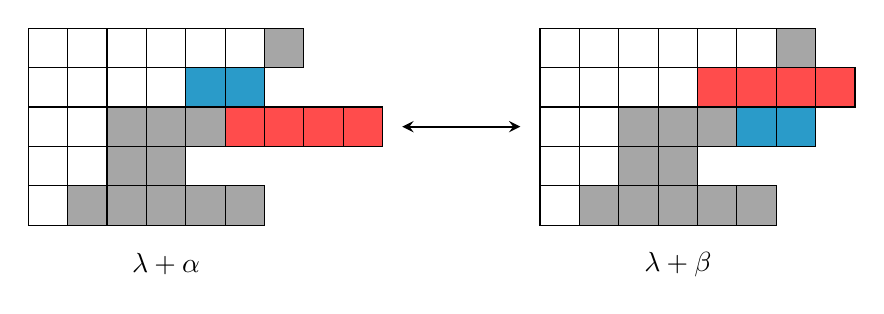
\begin{tikzpicture}[
                x=0.5cm, y=0.5cm,
                square/.style={draw, minimum size=0.5cm},
                white/.style={fill=white},
                gray/.style={fill=gray!70},
                blue/.style={fill=cyan!80!black},
                green/.style={fill=green!80!black},
                red/.style={fill=red!70!white}
            ]
            \begin{scope}[shift={(0,0)}]
                % First Row
                \foreach \x in {0,1,2,3,4,5} { \node[square, white] at (\x,4) {}; }
                \node[square, gray] at (6,4) {};
    
                % Second Row
                \foreach \x in {0,1,2,3} { \node[square, white] at (\x,3) {}; }
                \foreach \x in {4,5} { \node[square, blue] at (\x,3) {}; }
    
                % Third Row
                \foreach \x in {0,1} { \node[square, white] at (\x,2) {}; }
                \foreach \x in {2,3,4} { \node[square, gray] at (\x,2) {}; }
                \foreach \x in {5,6,7,8} { \node[square, red] at (\x,2) {}; }
    
                % Fourth Row
                \foreach \x in {0,1} { \node[square, white] at (\x,1) {}; }
                \foreach \x in {2,3} { \node[square, gray] at (\x,1) {}; }
    
                % Fifth Row
                \node[square, white] at (0,0) {};
                \foreach \x in {1,2,3,4,5} { \node[square, gray] at (\x,0) {}; }
            \end{scope}
            \node at (3, -1.5) {$\lambda + \alpha$};
            \begin{scope}[shift={(13,0)}] % Position of the second grid
                % First Row
                \foreach \x in {0,1,2,3,4,5} { \node[square, white] at (\x,4) {}; }
                \node[square, gray] at (6,4) {};
    
                % Second Row
                \foreach \x in {0,1,2,3} { \node[square, white] at (\x,3) {}; }
                \foreach \x in {4,5,6,7} { \node[square, red] at (\x,3) {}; }
    
                % Third Row
                \foreach \x in {0,1} { \node[square, white] at (\x,2) {}; }
                \foreach \x in {2,3,4} { \node[square, gray] at (\x,2) {}; }
                \foreach \x in {5,6} { \node[square, blue] at (\x,2) {}; }
    
                % Fourth Row
                \foreach \x in {0,1} { \node[square, white] at (\x,1) {}; }
                \foreach \x in {2,3} { \node[square, gray] at (\x,1) {}; }
    
                % Fifth Row
                \node[square, white] at (0,0) {};
                \foreach \x in {1,2,3,4,5} { \node[square, gray] at (\x,0) {}; }
            \end{scope}
            \node at (16, -1.5) {$\lambda + \beta$};
            \draw[<->, thick, >=stealth] (9,2) -- (12,2) node[midway, above] {};
    
        \end{tikzpicture}
        \caption{Example of the involution in the proof of Pieri's \(h\)-formula.}
        \label{fig:pieri-h-formula-involution}
    \end{figure}
    
    This map from \(\mathcal{B}\) to itself is an involution,
    and it satisfies that
        \(\lambda + \alpha + \delta_n\)
        \(\lambda + \beta + \delta_n\)
    differ by one transposition,
    hence
    \begin{equation}
        \tilde{a}_{\lambda + \alpha + \delta_n} + \tilde{a}_{\lambda + \beta + \delta_n} = 0.
    \end{equation}
    Finally,
    this implies that
    \begin{equation}
        \sum_{\alpha \in \mathcal{B}}
        \tilde{a}_{\lambda + \alpha + \delta_n}
        = 0,
    \end{equation}
    and consequently
    \begin{align}
        \tilde{a}_{\lambda + \delta_n} h_k
        &= \sum_{\substack{\text{compositions } \alpha \\ \text{of } k \text{ with length } n \\ (\lambda + \alpha) \setminus \lambda \text{ is a horizontal strip}}}
        \tilde{a}_{\lambda + \alpha + \delta_n} \\
        &= \sum_{\substack{\text{partitions } \mu \\ \lambda \setminus \mu \text{ is a Horizontal strip of size } k}}
        \tilde{a}_{\mu + \delta_n}.
    \end{align}
    Therefore,
    \begin{equation}
        a_\lambda h_k = \sum_{\mu} a_{\mu},
    \end{equation}
    where the sum is over all partitions \(\mu\) obtained by adding a horizontal strip of size \(k\) to \(\lambda\).
    Finally, the result follows by dividing by \(v_n\).
\end{proof}

In the next section, we solve a problem that we didn't even know we wanted to solve:
\emph{How to write \(h_\lambda\) and \(e_\lambda\) in the Schur basis?}

\section{Tableaux and Kostka Numbers}

\begin{definition}[Semistandard Young tableaux]
    A \vocab{semistandard tableaux \(T\)} 
    is a sequence of nested partitions
    \begin{equation}
        \varnothing = \lambda^{(0)}
        \subset \lambda^{(1)}
        \subset \cdots
        \subset \lambda^{(\ell)},
    \end{equation}
    such that \(\lambda^{(k)} \setminus \lambda^{(k-1)}\) is a horizontal strip, for all \(k \in \interval{\ell}\).
    We say that \(T\) has \vocab{shape} \(\lambda = \lambda^{(\ell)}\).
\end{definition}

Traditionally, a semistandard tableau \(T\) of shape \(\lambda\) is represented by filling the boxes of the diagram of \(\lambda\) with numbers from the set \(\{1, 2, \ldots, \ell\}\). Specifically, the number \(i\) is placed in the boxes corresponding to the horizontal strip \(\lambda^{(i)} \setminus \lambda^{(i-1)}\).

Under this depiction, a filling of the boxes of a Young diagram is semistandard if and only if the entries in each row are weakly increasing from left to right, and the entries in each column are strictly increasing from top to bottom.

\begin{example}
    Consider the following semistandard tableaux of shape \(\composition{5, 4, 2}\):
    \begin{equation}
        \varnothing
        \subset \composition{3}
        \subset \composition{4, 2}
        \subset \composition{4, 2}
        \subset \composition{5, 4}
        \subset \composition{5, 4, 2}.
    \end{equation}
    This tableaux is drawn as
    \begin{equation}
        \begin{ytableau}
            1 & 1 & 1 & 2 & 4 \\
            2 & 2 & 4 & 4 \\
            5 & 5
        \end{ytableau}.
    \end{equation}
\end{example}

The \vocab{weight} (sometimes called \vocab{content}) of a tableaux
is the composition \(\alpha\) such that the number \(i\) appears \(\alpha_i\) times in the tableaux, that is, \(\alpha_i\) is the size of the horizontal strip \(\lambda^{(i)} \setminus \lambda^{(i-1)}\).

\begin{definition}[Standard Young tableaux]
    A \vocab{standard tableaux} is a semistandard Young tableaux with weight \(\composition{1, 1, \ldots, 1}\), that is, each horizontal strip has size \(1\).
\end{definition}

\begin{definition}[Kostka numbers]
    Let \(\lambda\) be a partition and \(\alpha\) be a composition.
    The \vocab{Kostka number} \(K_{\lambda \alpha}\) is the number of standard Young tableaux of shape \(\lambda\) and weight \(\alpha\).
\end{definition}

\begin{theorem} \label{thm:h-e-sum-kostka-schur}
    Let \(\alpha\) be a composition.
    Then,
    \begin{equation}
        h_\alpha = \sum_{\lambda} K_{\lambda \alpha} \schur{\lambda},
    \end{equation}
    and
    \begin{equation}
        e_\alpha = \sum_{\lambda} K_{\lambda \alpha} \schur{\tilde\lambda}.
    \end{equation}
\end{theorem}

\begin{proof}
    Note that 
    \begin{align}
        h_\alpha
        &= h_{\alpha_1} h_{\alpha_2} \cdots h_{\alpha_\ell} \\
        &= \schur{\varnothing} h_{\alpha_1} \schur{\varnothing} h_{\alpha_2} \cdots \schur{\varnothing} h_{\alpha_\ell},
    \end{align}
    and then the result follows by successively applying \nameref{thm:pieri-h-formula}.
    The proof for the \(e\)-formula is similar, using \nameref{thm:pieri-e-formula}.
\end{proof}

We list some observations about Kostka numbers.

\begin{corollary} \label{cor:kostka-composition-sort}
    Let \(\alpha\) be a composition and let \(\mu = \overline{\alpha}\).
    Then, \(K_{\lambda \alpha} = K_{\lambda \mu}\).
\end{corollary}

\begin{proof}
    Since \(h_\alpha = h_\mu\), the result follows from Theorem~\ref{thm:h-e-sum-kostka-schur} and the fact that the Schur polynomials are linearly independent.
\end{proof}

\begin{fact}
    If \(|\lambda| \neq |\mu|\), then \(K_{\lambda \mu} = 0\).
\end{fact}

\begin{fact}
    Let \(\lambda\) be a partition.
    Then \(K_{\lambda \lambda} = 1\).
\end{fact}

The only standard Young tableaux of shape \(\lambda\) and weight \(\lambda\) is the one where the number \(i\) is placed in the \(i\)\textsuperscript{th} box of the \(i\)\textsuperscript{th} row.
This tableaux is called \vocab{Yamanouchi tableaux}, \vocab{the highest weight tableaux of shape \(\lambda\)}, or \vocab{supersemistandard tableaux}.

\begin{fact}
    Let \(\lambda, \mu\) be partitions.
    If \(K_{\lambda \mu} \neq 0\), then \(\lambda \geq \mu\).
\end{fact}

\begin{proof}
    Let \(i\) be a positive integer.
    The entries of a standard Young tableaux of shape \(\lambda\) and weight \(\mu\) that are at most \(i\) must be contained in the first \(i\) rows of the Young diagram of \(\lambda\).
    Therefore, \(\lambda_1 + \cdots + \lambda_i \geq \mu_1 + \cdots + \mu_i\) for all \(i\),
    and consequently, \(\lambda \geq \mu\).
\end{proof}

\begin{fact}
    Kostka numbers are not symmetric, that is, 
    there exist partitions \(\lambda, \mu\) such that \(K_{\lambda \mu} \neq K_{\mu \lambda}\).
\end{fact}

\begin{example}
    Let \(\lambda = \composition{2}\) and \(\mu = \composition{1, 1}\).
    Then, \(K_{\lambda \mu} = 1\) and \(K_{\mu \lambda} = 0\).
\end{example}

The \vocab{Kostka matrix} \(K\) is the matrix where the entry in the \(\mu\)\textsuperscript{th} row and \(\lambda\)\textsuperscript{th} column is \(K_{\lambda \mu}\) (note the reversal of indices).
Note that \(K\) is upper triangular (with respect a linear extension of the dominance order) and its diagonal entries are all \(1\).
Therefore, \(K\) is invertible, and its inverse has integer entries.
We call \(K^{-1}\) the \vocab{inverse Kostka matrix}.
Let \(K^{-1}_{\lambda \mu}\) be the entry in the \(\mu\)\textsuperscript{th} row and \(\lambda\)\textsuperscript{th} column of \(K^{-1}\).

\begin{theorem}
    Let \(\lambda\) be a partition.
    Then,
    \begin{equation}
        \omega(\schur{\lambda}) = \schur{\tilde\lambda}.
    \end{equation}
\end{theorem}

\begin{proof}
    Theorem~\ref{thm:h-e-sum-kostka-schur} implies that
    \begin{equation}
        \schur{\lambda} = \sum_{\mu} K_{\lambda \mu}^{-1} h_\mu,
    \end{equation}
    and 
    \begin{equation}
        \schur{\tilde\lambda} = \sum_{\mu} K_{\lambda \mu}^{-1} e_\mu.
    \end{equation}
    It is straightforward to check that applying \(\omega\) to the right-hand side of the first equation gives the right-hand side of the second equation, and the result follows.
\end{proof}

\begin{theorem}[Jacobi--Trudi's determinant formula] \label{thm:jacobi-trudi}
    Let \(\lambda\) be a partition and let \(n \geq \ell(\lambda)\) be an integer.
    Then,
    \begin{equation}
        \schur{\lambda} = \det\left( h_{\lambda_i + n - i - j} \right)_{i, j \in \interval{n}}.
    \end{equation}
    and
    \begin{equation}
        \schur{\tilde\lambda} = \det\left( e_{\lambda_i + n - i - j} \right)_{i, j \in \interval{n}}.
    \end{equation}
\end{theorem}

\begin{example}
    Let's compute \(\schur{\composition{3, 1}}\) using \nameref{thm:jacobi-trudi}.
    Let \(n = 4\).
    We have
    \begin{equation}
        \schur{\composition{3, 1}}
        = \left|
            \begin{matrix}
                h_3 & h_4 & h_5 & h_6 \\
                h_0 & h_1 & h_2 & h_3 \\
                0   & 0   & h_0 & h_1 \\
                0   & 0   & 0   & h_0
            \end{matrix}
        \right|
        = \left|
            \begin{matrix}
                h_3 & h_4 \\
                h_0 & h_1 \\
            \end{matrix}
        \right|
        = h_{\composition{3, 1}} - h_{\composition{4}},
    \end{equation}
    and
    \begin{equation}
        \schur{\composition{3, 1}} = \schur{\tilde{\composition{2, 1, 1}}} =
        \left|
            \begin{matrix}
                e_2 & e_3 & e_4 \\
                e_0 & e_1 & e_2 \\
                0   & e_0 & e_1
            \end{matrix}
        \right|
        = e_{\composition{2, 1, 1}} + e_{\composition{4}} - e_{\composition{3, 1}} - e_{\composition{2, 2}}.
    \end{equation}
\end{example}

\begin{proof}[Proof of \nameref{thm:jacobi-trudi}]
    It is straightforward to check that the determinants are equal for all \(n \geq \ell(\lambda)\). Therefore, it suffices to prove the result for \(n = \ell(\lambda)\).

    We proceed by induciton on \(n = \ell(\lambda)\).
    The result is true for \(n = 0\).

    We column expand along the rightmost column
    \begin{equation}
        \det\left( \schur{\lambda_i + \ell - i - j} \right)_{i, j \in \interval{n}}
        =
        \sum_{i=1}^\ell
        (-1)^{\ell - i}
        h_{\lambda_i + \ell - i}
        \schur{\composition{\lambda_1, \ldots, \lambda_{i-1}, \lambda_{i+1} - 1, \ldots, \lambda_\ell - 1}}
    \end{equation}

    \textcolor{red}{... I did not finish this proof. Reading a book proof might be better.}
\end{proof}

\begin{theorem}
    \begin{equation}
        \prod_{i, j} (1 - x_i y_j)^{-1} = \sum_{\lambda} \schur{\lambda}(x) \schur{\lambda}(y).
    \end{equation}
\end{theorem}

\begin{proof}
    By \nameref{thm:jacobi-trudi}, we have
    \begin{equation}
        \schur{\lambda} = \sum_{w \in \sym{n}} \sign(w) h_{\lambda + \delta - w \cdot \delta}.
    \end{equation}
    Multiplying by \(v_n\) gives
    \begin{equation}
        a_\lambda = a_\varnothing \sum_{w \in \sym{n}} \sign(w) h_{\lambda + \delta - w \cdot \delta}.
    \end{equation}
    Let \(\alpha = \lambda + \delta\).
    Then,
    \begin{equation}
        \tilde{a}_\alpha = \tilde{a}_\delta \sum_{w \in \sym{n}} \sign(w) h_{\alpha - w \cdot \delta}.
    \end{equation}

    Now, recall that
    \begin{equation}
        \prod_{i, j} (1 - x_i y_j)^{-1} = \sum_{\lambda} h_\lambda(x) m_\lambda(y) = \sum_{\gamma} h_{\overleftarrow{\gamma}}(x) x^\gamma,
    \end{equation}
    and consequently
    \begin{align}
        \tilde{a}_\delta(x) \tilde{a}_\delta(y) 
        \prod_{i, j} (1 - x_i y_j)^{-1}
        &= \tilde{a}_\delta(x) \sum_{\gamma} \sum_{w \in \sym{n}} \sign(w) h_{\overleftarrow{\gamma}}(x) y^{\gamma} \\
        &= \textcolor{red}{... TBD}.
    \end{align}
\end{proof}

\begin{corollary}
    Let \(\lambda, \mu\) be partitions.
    Then,
    \begin{equation}
        \langle \schur{\lambda}, \schur{\mu} \rangle = \delta_{\lambda \mu}.
    \end{equation}
\end{corollary}

\begin{corollary} \label{cor:schur-sum-kostka-m}
    Let \(\lambda\) be a partition.
    Then,
    \begin{equation}
        \schur{\lambda} = \sum{\mu} K_{\lambda \mu} m_\mu.
    \end{equation}
\end{corollary}

\begin{proof}
    Define \(Q_{\lambda, \xi}\) so that \(\schur{\lambda} = \sum{\xi} Q_{\lambda, \xi} m_\xi\).
    On the one hand, we have
    \begin{equation}
        \langle h_\mu, \schur{\lambda} \rangle
        = \langle h_\mu, \sum_{\xi} Q_{\lambda, \xi} m_\xi \rangle
        = \sum_{\xi} Q_{\lambda, \xi} \langle h_\mu, m_\xi \rangle
        = Q_{\lambda, \mu}.
    \end{equation}
    On the other hand, we have
    \begin{equation}
        \langle h_\mu, \schur{\lambda} \rangle
        = \langle \sum_{\nu} K_{\nu \mu} \schur{\nu}, \schur{\lambda} \rangle
        = \sum_{\nu} K_{\nu \mu} \langle \schur{\nu}, \schur{\lambda} \rangle
        = K_{\lambda \mu}.
    \end{equation}
    Therefore, \(Q_{\lambda, \mu} = K_{\lambda \mu}\), and the result follows.
\end{proof}

\begin{example}[\(\schur{\composition{2, 1}}\)]
    Let's compute \(\schur{\composition{2, 1}}\) using Corollary~\ref{cor:schur-sum-kostka-m}.
    We have
    \begin{equation}
        \schur{\composition{2, 1}}
        =
        0 m_{\composition{3}} + 
        1 m_{\composition{2, 1}} +
        2 m_{\composition{1, 1, 1}}.
    \end{equation}
\end{example}

\begin{example}[\(\schur{\composition{4, 2}}\)]
    Let's compute \(\schur{\composition{4, 2}}\) using Corollary~\ref{cor:schur-sum-kostka-m}.
    We have
    \begin{equation}
        \schur{\composition{4, 2}}
        =
        1 m_{\composition{4, 2}} +
        1 m_{\composition{4, 1, 1}} +
        1 m_{\composition{3, 3}} +
        2 m_{\composition{3, 2, 1}} +
        3 m_{\composition{3, 1, 1, 1}} +
        3 m_{\composition{2, 2, 2}} +
        6 m_{\composition{2, 2, 1, 1}} +
        4 m_{\composition{2, 1, 1, 1, 1}} +
        9 m_{\composition{1, 1, 1, 1, 1, 1}}.
    \end{equation}
\end{example}

From Corollary~\ref{cor:schur-sum-kostka-m}, we can observe that, for all nonnegative integers \(k\),
\begin{equation}
    \schur{\composition{1}^k} = e_k
    \qquad \text{and} \qquad
    \schur{\composition{k}} = h_k.
\end{equation}

\begin{corollary}
    Let \(\lambda\) be a partition.
    Then,
    \begin{equation}
        \schur{\lambda} = \sum_{\text{semistandard tableaux } T \text{ of shape } \lambda} x^{\wt(T)},
    \end{equation}
    where \(\wt(T)\) is the weight of \(T\).
\end{corollary}

\begin{proof}
    By Corollary~\ref{cor:schur-sum-kostka-m}, we have
    \begin{equation}
        \schur{\lambda} = \sum_{\mu} K_{\lambda \mu} m_{\mu}
        = \sum_{\alpha} K_{\lambda \alpha} x^{\alpha}
        = \sum_{\text{semistandard tableaux } T \text{ of shape } \lambda} x^{\wt(T)}. \qedhere
    \end{equation}
\end{proof}

We provide a combinatorial proof of Corollary~\ref{cor:kostka-composition-sort}, restated below.
\begin{fact}
    Let \(\alpha\) and \(\beta\) be compositions such that \(\overline{\alpha} = \overline{\beta} = \mu\).  Then, \(K_{\lambda \alpha} = K_{\lambda \beta}\).
\end{fact}
\begin{proof}[Proof by Bender--Knuth, 1972]
    By induction, it suffices to show that the result is true when \(\alpha\) and \(\beta\) differ by swapping coordinates \(i\) and \(i+1\).
    Define the \vocab{\(i\)\textsubscript{th} Bender--Knuth involution}
    \begin{equation}
        \BK{i} \colon SSYT(\mu) \to SSYT(\mu)
    \end{equation}
    as follows.
    If entries \(i\) and \(i+1\) are in the column, we say that these labels are \emph{frozen}.
    The remaining entries \(i\) and \(i+1\) are said to be \emph{free}.
    It is straightforward to check that, in each row, the free entries look like
    \begin{equation}
        \ytableausetup{boxsize=1cm}
        \begin{ytableau}
            i & i & \cdots & i & i+1 & i+1 & \cdots & i+1
        \end{ytableau}.
    \end{equation}
    Suppose row \(k\) has \(a\) free entries \(i\) and \(b\) free entries \(i+1\).
    The involution \(\BK{i}\) swaps those entires to \(b\) entries \(i\) and \(a\) entries \(i+1\).
    In other words, the middle \(|a-b|\) free entries are swapped.
    By doing this to all rows, we obtain a bijection between the set of semistandard tableaux of shape \(\lambda\) and weight \(\alpha\) and the set of semistandard tableaux of shape \(\lambda\) and weight \(\beta\), and the result follows.
\end{proof}

\begin{remark}
    The Bender--Knuth involutions do not satisfy braid relations,
    and therefore they do not generate the symmetric group.
    Instead, we get elements that satisfy
    \begin{gather}
        \BK{i}^2 = \id, \\
        \BK{i} \BK{j} = \BK{j} \BK{i} \quad \text{if } |i - j| > 1, \\
        (\BK{1} \BK{2})^6 = \id,
    \end{gather}
    and, by letting \(q_i =
    \BK{1}
    (\BK{2} \BK{1})
    (\BK{3} \BK{2} \BK{1})
    \cdots
    (\BK{i} \cdots \BK{2} \BK{1})\),
    we get that, for \(i \geq 2\),
    \begin{equation}
        (\BK{i} q_i)^4 = \id.
    \end{equation}
    There are more relations, but nobody knows the entire list.
\end{remark}

\begin{definition} \label{def:skew-schur}
    Let \(\lambda \subset \nu\) be partitions.
    The \vocab{skew Schur polynomial} is defined as
    \begin{equation}
        \schur{\nu / \lambda} = \sum_{\text{semistandard tableaux } T \text{ of skew shape } \nu / \lambda} x^{\wt(T)}.
    \end{equation}
\end{definition}

Note that any schur polynomial is a skew Schur polynomial, by taking \(\lambda = \varnothing\).
Hence, many results about Schur polynomials can be generalized to skew Schur polynomials.

\begin{theorem} \label{thm:skew-schur-symmetric}
    Let \(\lambda \subset \mu\) be partitions.
    Then, \(\schur{\nu / \lambda}\) is a symmetric function.
\end{theorem}

Theorem~\ref{thm:skew-schur-symmetric} follows from applying Bender--Knuth involutions to semistandard tableaux of skew shape.

\section{The exponential specialization}

Recall \(\Sym = \rationals[p_1, p_2, \ldots]\).
Define
\begin{equation}
    \operatorname{ex} \colon \Sym \to \rationals[t]
\end{equation}
by
\begin{align*}
    p_1 &\mapsto t, \\
    p_k &\mapsto 0 \quad \text{for } k \geq 2.
\end{align*}

\begin{proposition}
    Let \(f \in \Sym\).
    Then,
    \begin{equation}
        \operatorname{ex}(f)
        = \sum_{n=0}^\infty \left( [x_1x_2\dots x_n] f \right) \frac{t^n}{n!},
    \end{equation}
    that is, \(\operatorname{ex}(f)\) is the exponential generating function of square-free coefficients of \(f\).
\end{proposition}

\begin{proof}
    Both sides are linear in \(f\), so it suffices to check the result for the elements of a basis of \(\Sym\).
    We check that the result is true for \(f = p_\lambda\), where \(\lambda\) is a partition.

    If \(\lambda \neq \composition{1}^k\) for all \(k\), then both sides are zero.
    If \(\lambda = \composition{1}^k\), then
    \begin{equation}
        \operatorname{ex}(p_{\composition{1}^k}) = (\operatorname{ex}(p_1))^k = t^k
    \end{equation}
    and
    \begin{equation}
        \sum_{n=0}^\infty \left( [x_1x_2\dots x_n] p_{\composition{1}^k} \right) \frac{t^n}{n!}
        = \left( [x_1x_2\dots x_k] p_{\composition{1}^k} \right) \frac{t^k}{k!}
        = k! \frac{t^k}{k!}
        = t^k,
    \end{equation}
    and the result follows.
\end{proof}

\begin{corollary}
    Let \(f \in \Sym_k\),
    with \(f = \sum_{\lambda} c_\lambda m_\lambda\).
    Then,
    \begin{equation}
        \operatorname{ex}(f) = c_{\composition{1}^k}.
    \end{equation}
\end{corollary}

\begin{corollary}
    Let \(\lambda\) be a partition.
    Then,
    \begin{equation}
        \operatorname{ex}(p_\lambda) =
        \begin{cases}
            t^k & \text{if } \lambda = \composition{1}^k, \\
            0 & \text{otherwise}.
        \end{cases}
    \end{equation}
\end{corollary}

\begin{corollary}
    Let \(\lambda\) be a partition.
    Then,
    \begin{equation}
        \operatorname{ex}(m_\lambda) =
        \begin{cases}
            \frac{t^n}{n!} & \text{if } \lambda = \composition{1}^k, \\
            0 & \text{otherwise}.
        \end{cases}
    \end{equation}
\end{corollary}

\begin{corollary}
    Let \(\lambda\) be a partition.
    Then,
    \begin{equation}
        \operatorname{ex}(h_\lambda) = \operatorname{ex}(e_\lambda) = 
        \frac{1}{\lambda_1! \lambda_2! \cdots} t^{|\lambda|}.
    \end{equation}
\end{corollary}

\begin{corollary}
    Let \(\lambda \subset \nu\) be partitions.
    Then,
    \begin{equation}
        \operatorname{ex}(\schur{\nu / \lambda}) =
        \frac{f^{\nu / \lambda}}{| \nu / \lambda |!} t^{|\nu / \lambda|},
    \end{equation}
    where \(f^{\nu / \lambda}\) is the number of standard Young tableaux of skew shape \(\nu / \lambda\).
\end{corollary}

\section{Skew Schur polynomials}

Let \(\lambda \subset \nu\) and let \(\alpha\) be a composition.
The \vocab{skew Kostka number} \(K_{\nu / \lambda, \alpha}\) is the number of standard Young tableaux of skew shape \(\nu / \lambda\) and weight \(\alpha\).

Then, 
\begin{equation}
    \schur{\nu / \lambda} = \sum_{\mu} K_{\nu / \lambda, \mu} m_\mu.
\end{equation}

Therefore,
\begin{equation}
    \left\langle \schur{\nu / \lambda}, h_\mu \right\rangle = K_{\nu / \lambda, \mu}.
\end{equation}

\begin{theorem}
    Let \(\lambda, \nu\) be partitions.
    Then,
    \begin{equation}
        \schur{\lambda}^\perp \schur{\nu} =
        \begin{cases}
            \schur{\nu / \lambda} & \text{if } \lambda \subset \nu, \\
            0 & \text{otherwise}.
        \end{cases}
    \end{equation}
\end{theorem}

\begin{proof}
    Let \(\mu\) be a partition.
    Then,
    \begin{equation}
        \left\langle \schur{\lambda}^\perp \schur{\nu}, h_\mu \right\rangle
        = \left\langle \schur{\lambda}, \schur{\nu} h_\mu \right\rangle
        = K_{\nu / \lambda, \mu}
        =
        \begin{cases}
            \left\langle \schur{\nu / \lambda}, h_\mu \right\rangle & \text{if } \lambda \subset \nu, \\
            0 & \text{otherwise}.
        \end{cases}
    \end{equation}
    The result follows by linearity.
\end{proof}

\begin{corollary}
    Let \(\lambda, \mu, \nu\) be partitions.
    Then,
    \begin{equation}
        \left\langle \schur{\lambda} \schur{\mu}, \schur{\nu} \right\rangle
        = \left\langle \schur{\lambda}, \schur{\nu / \mu} \right\rangle.
        = \left\langle \schur{\mu}, \schur{\nu / \lambda} \right\rangle.
    \end{equation}
\end{corollary}

Let \(\lambda, \mu, \nu\) be partitions.
Define the \vocab{Littlewood--Richardson coefficient} \(c_{\lambda \mu}^\nu\) by
\begin{equation}
    c_{\lambda \mu}^\nu = \left\langle \schur{\lambda} \schur{\mu}, \schur{\nu} \right\rangle.
\end{equation}
Since the Schur polynomials are orthonormal, we have
\begin{equation}
    \schur{\lambda} \schur{\mu} = \sum{\nu} c_{\lambda \mu}^\nu \schur{\nu}.
\end{equation}
and
\begin{equation}
    \schur{\nu / \lambda} = \sum{\mu} c_{\nu / \lambda, \mu} \schur{\mu}.
\end{equation}
We know that these coefficients are integers.

From the equations above, we can think of two ways to attempt to compute the Littlewood--Richardson coefficients:
\begin{itemize}
    \item \emph{product of tableaux:} start with tableaux \(T_\lambda\) and \(T_\mu\) and try to build a tableau \(T_\nu\). 
    \item \emph{rectification of tableau:} start with a tableau \(T_{\nu / \lambda}\) and try to build a tableau \(T_\mu\).
\end{itemize}

For a tableau \(T\),
write \(^aT^b\) for the subtableau of \(T\) of columns \(a\) through \(b\).

\begin{theorem} \label{thm:skew-tilde-a}
    Let \(\lambda, \nu, \mu\) be partitions such that \(\nu \subset \mu\).
    Then,
    \begin{equation}
        \tilde{a}_{\lambda + \delta} \schur{\mu/\nu}
        =
        \sum \tilde{a}_{\lambda + \wt(T) + \delta}
    \end{equation}
    where the sum is over all tableaux \(T\) of shape \(\mu/\nu\)
    such that \(\lambda + \wt(^jT^\infty)\) is a partition for all \(j\).
\end{theorem}

\begin{proof}[Proof (Stembridge, 2002)]
    We expand the definitions of \(\tilde{a}\) and \(\schur{\mu/\nu}\),
    use the fact that the Schur polynomials are symmetric,
    \begin{align}
        \tilde{a}_{\lambda + \delta} \schur{\mu/\nu}
        &= 
        \sum_{w \in \sym{n}}
        \sum_{T \in \SSYT(\mu/\nu)}
        \sign(w) x^{w(\lambda + \delta) + \wt(T)} \\
        &=
        \sum_{w \in \sym{n}}
        \sum_{T \in \SSYT(\mu/\nu)}
        \sign(w) x^{w(\lambda + \delta + \wt(T))} \\
        &=
        \sum_{T \in \SSYT(\mu/\nu)}
        \sum_{w \in \sym{n}}
        \sign(w) x^{w(\lambda + \wt(T)) + \delta} \\
        &=
        \sum_{T \in \SSYT(\mu/\nu)}
        \tilde{a}_{\lambda + \wt(T) + \delta}.
    \end{align}

    Let \(\mathcal{B}\) be the set of semistandard tableaux \(T\) of shape \(\mu/\nu\) such that \(\lambda + \wt(^jT^\infty)\) is not a partition for some \(j\).

    Let \(T \in \mathcal{B}\), and let \(j\) be maximal such that \(\lambda + \wt(^jT^\infty)\) is not a partition.
    Then, there exists a minimum \(k\) such that
    \begin{equation}
        \lambda_k + (\wt(^jT^\infty))_k > \lambda_{k+1} + (\wt(^jT^\infty))_{k+1}.
    \end{equation}
    Since \(\lambda + \wt(^{j+1}T^\infty)\) is a partition, we have
    \begin{equation}
        \lambda_k + (\wt(^{j+1}T^\infty))_k \leq \lambda_{k+1} + (\wt(^{j+1}T^\infty))_{k+1}.
    \end{equation}
    Moreover, the \(j\)\textsuperscript{th} column of \(T\) contains distinct entries.
    Therefore, the \(j\)\textsuperscript{th} column of \(T\) contains one entry \(k\), it contains no entry \(k+1\), and
    \begin{equation} \label{eq:skew-tilde-a-1}
        \lambda_k + (\wt(^jT^\infty))_k = \lambda_{k+1} + (\wt(^jT^\infty))_{k+1} + 1.
    \end{equation}

    Let \(T^*\) be obtained from \(T\) by applying the Bender--Knuth involution \(\BK{k}\) only to \(^1T^{j-1}\).
    Note that \(T^*\) is still in \(\mathcal{B}\),
    and moreover, \((T^*)^* = T\).
    Therefore, this is an involution on \(\mathcal{B}\).

    Note that
    \begin{equation} \label{eq:skew-tilde-a-2}
        \wt(^1(T^*)^{j-1}) = s_k \wt(^1T^{j-1})
    \end{equation}
    and
    \begin{equation} \label{eq:skew-tilde-a-3}
        \wt(^jT^\infty) = \wt(^j(T^*)^\infty).
    \end{equation}
    From Equations~\eqref{eq:skew-tilde-a-1}, \eqref{eq:skew-tilde-a-2}, and \eqref{eq:skew-tilde-a-3}, we find that
    \begin{equation}
        \lambda + \wt(T^*) + \delta = s_k(\lambda + \wt(T) + \delta).
    \end{equation}
    Therefore,
    \begin{equation}
        \tilde{a}_{\lambda + \wt(T) + \delta}
        =
        - \tilde{a}_{\lambda + \wt(T^*) + \delta},
    \end{equation}
    which implies that
    \begin{equation}
        \sum_{T \in \mathcal{B}} \tilde{a}_{\lambda + \wt(T) + \delta} = 0.
    \end{equation}

    Therefore, as desired,
    \begin{equation}
        \tilde{a}_{\lambda + \delta} \schur{\mu/\nu}
        =
        \sum_{T \in \SSYT(\mu/\nu) \setminus \mathcal{B}}
        \tilde{a}_{\lambda + \wt(T) + \delta}.
    \end{equation}
\end{proof}

Note that Theorem~\ref{thm:skew-tilde-a} recovers the definition of Schur polynomials.

\begin{corollary}
    Let \(\mu\) be a partition.
    Then,
    \begin{equation}
        \tilde{a}_{\delta} \schur{\mu} = \tilde{a}_{\mu + \delta}.
    \end{equation}
\end{corollary}

\begin{proof}
    We know
    \begin{equation}
        \tilde{a}_{\delta} \schur{\mu} = \sum{T} \tilde{a}_{\wt(T) + \delta},
    \end{equation}
    where the sum is over all tableaux \(T\) of shape \(\mu\) such that \(\wt(^jT^\infty)\) is a partition for all \(j\),
    but there is only one such tableau, the Yamanouchi tableau of shape \(\mu\),
    and the result follows.
\end{proof}

\begin{corollary}[Zelevinsky] \label{cor:zelevinsky}
    Let \(\lambda, \mu, \nu\) be partitions.
    Then,
    \begin{equation}
        \schur{\lambda} \schur{\mu / \nu} =
        \sum \schur{\lambda + \wt(T)},
    \end{equation}
    where the sum is over all tableaux \(T\) of shape \(\mu/\nu\) such that \(\lambda + \wt(^jT^\infty)\) is a partition for all \(j\).
\end{corollary}

\begin{proof}
    Obtained from Theorem~\ref{thm:skew-tilde-a} by dividing by the Vandermonde determinant \(\tilde{a}_\delta\).
\end{proof}

\begin{corollary}
    Let \(\mu, \nu\) be partitions.
    Then,
    \begin{equation}
        \schur{\mu / \nu} = \sum \schur{\mu + \wt(T)},
    \end{equation}
    where the sum is over all tableaux \(T\) of shape \(\mu/\nu\) such that \(\wt(^jT^\infty)\) is a partition for all \(j\).
\end{corollary}

\begin{proof}
    Obtained from Corollary~\ref{cor:zelevinsky} by setting \(\lambda = \varnothing\).
\end{proof}

\begin{corollary}
    Let \(\lambda, \mu\) be partitions.
    Then,
    \begin{equation}
        \schur{\lambda} \schur{\mu} = \sum \schur{\lambda + \wt(T)},
    \end{equation}
    where the sum is over all tableaux \(T\) of shape \(\mu\) such that \(\lambda + \wt(^jT^\infty)\) is a partition for all \(j\).
\end{corollary}

\begin{proof}
    Obtained from Corollary~\ref{cor:zelevinsky} by setting \(\nu = \varnothing\).
\end{proof}

\begin{example}
    Let \(\lambda = \mu = \composition{2, 1}\).
    Then, the desired sum is over all tableaux of shape \(\composition{2, 1}\) such that \(\composition{2, 1, 0, 0, 0} + \wt(^jT^\infty)\) is a partition for all \(j\).
    These tableaux are
    \begin{gather}
        \ytableausetup{boxsize=1em}
        \ytableaushort{11,2}, \quad
        \ytableaushort{11,3}, \quad
        \ytableaushort{12,2}, \quad
        \ytableaushort{12,3}, \quad
        \ytableaushort{13,2}, \quad
        \ytableaushort{13,4}, \quad
        \ytableaushort{23,3}, \quad
        \ytableaushort{23,4}, \quad
        \ytableaushort{23,4}.
    \end{gather}
    and consequently
    \begin{equation}
        \schur{\composition{2, 1}} \schur{\composition{2, 1}}
        =
        \schur{\composition{4, 2}} +
        \schur{\composition{4, 1, 1}} +
        \schur{\composition{3, 3}} +
        2\schur{\composition{3, 2, 1}} +
        \schur{\composition{3, 1, 1, 1}} +
        \schur{\composition{2, 2, 2}} +
        2\schur{\composition{2, 2, 1, 1}}.
    \end{equation}
\end{example}

Given a word \(a = a_1 a_2 \cdots a_n\),
we say that this word satisfies the \vocab{Yamanouchi condition} if,
for all partial words \(a_1 a_2 \cdots a_k\),
the number of entries \(i\) is at least as large as the number of entries \(i+1\).

Note that \(T\) satisfies \(\lambda + \wt(^jT^\infty)\) is a partition for all \(j\) if and only if the tableau
\begin{equation}
    T \star Y_\lambda = 
    \vcenter{\hbox{
    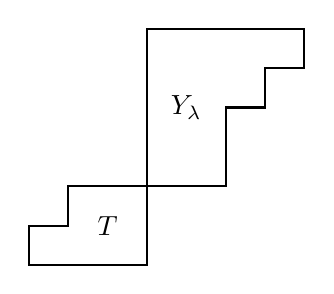
\begin{tikzpicture}[scale=.5, thick]
        \draw (0, 0) -- (2, 0) -- (2, 2) -- (3, 2) -- (3, 3) -- (4, 3) -- (4, 4) -- (0, 4) -- cycle;
        \draw (0, 0) -- (-2, 0) -- (-2, -1) -- (-3, -1) -- (-3, -2) -- (0, -2) -- cycle;
        \node at (1, 2) {\(Y_\lambda\)};
        \node at (-1, -1) {\(T\)};
    \end{tikzpicture}
    }}
\end{equation}
satisfies the \vocab{Yamanouchi condition},
namely,
when we read the columns of \(T \star Y_\lambda\) from right to left,
reading each column from top to bottom,
we obtain an Yamanouchi word.

\begin{example}
    Let's compute \(c_{\composition{2, 1} \composition{2, 1}}^{\composition{3, 2, 1}}\).
    We have
    \begin{equation}
        c_{\composition{2, 1} \composition{2, 1}}^{\composition{3, 2, 1}}
        = [\schur{\composition{2, 1}}] \schur{\composition{3, 2, 1} / \composition{2, 1}},
    \end{equation}
    which equals the number of tableaux of shape \(\composition{3, 2, 1} / \composition{2, 1}\) with weight \(\composition{2, 1}\) that satisfy the Yamanouchi condition.
    There are two such tableaux, namely,
    \begin{equation}
        \ytableaushort{\none\none1,\none1,2}, \quad
        \ytableaushort{\none\none1,\none2,1}.
    \end{equation}
    and therefore \(c_{\composition{2, 1} \composition{2, 1}}^{\composition{3, 2, 1}} = 2\).
\end{example}

\chapter{Tableaux Combinatorics}

In this chapter, we will reinvent the theory of Schur polynomials using tableaux combinatorics.
We will think of Schur polynomials as generating functions of weights of tableaux,
namely
\begin{equation}
    s_\lambda = \sum_{T \in \SSYT(\lambda)} x^{\wt(T)}.
\end{equation}

\section{Robinson--Schensted correspondence}

We know that
\begin{equation}
    \schur{\lambda} \schur{\composition{1}} = \sum{\mu : |\mu / \lambda| = 1} \schur{\mu}.
\end{equation}

Therefore, we have some hope that there exists a bijection
\begin{equation}
    \SSYT(\lambda) \times \positives \longleftrightarrow \bigsqcup_{\mu : |\mu / \lambda| = 1} \SSYT(\mu).
\end{equation}

Indeed, there exists a bijection called \vocab{row insertion} or \vocab{row bumping} or \vocab{Schensted insertion}.
Refer to \cite{Fulton1997} for the definition of this insertion algorithm.

Given \(T \in \SSYT(\lambda)\) and \(a \in \positives\),
we denote by \(T \leftarrow a\) the result of applying row inserting \(a\) into \(T\).

\begin{lemma}
    \(T \leftarrow a\) is a semistandard tableau.
\end{lemma}

\begin{proof}
    The fact that the rows are weakly increasing is immediate.

    If \(x\) is moved to a box \(b\),
    then either \(b\) was empty or it contained a larger entry \(y > x\).
    In the first case, \(b^{\downarrow}\) is empty, which is fine.
    In the second case, \(b^{\downarrow}\) contains a larger entry \(z > y\).
    Therefore, the entry in \(b\) is strictly smaller than the entry in \(b^{\downarrow}\).

    It is analogous to check that the entry in \(b^{\uparrow}\) is strictly smaller than the entry in \(b\).
\end{proof}

\begin{lemma}
    Let \(\lambda\) be a partition.
    Let \(U\) be a semistandard tableau of shape \(\mu\), where \(\mu / \lambda\) is one box.
    Then, there exists a unique semistandard tableau \(T\) of shape \(\lambda\) and a positive integer \(a\) such that \(T \leftarrow a = U\).
\end{lemma}

Refer to \cite{Fulton1997} for the proof of this lemma.

\begin{corollary} \label{cor:row-insertion-bijection}
    The row insertion map
    \begin{equation}
        \SSYT(\lambda) \times \positives \to \bigsqcup_{\mu : |\mu / \lambda| = 1} \SSYT(\mu)
    \end{equation}
    is a bijection, and moreover, the weight of \(T \leftarrow a\) is \(\wt(T) + \wt\left( \boxed{a} \right)\).
\end{corollary}

\begin{proof}
    The bijection is immediate from the previous lemmas.
    The weight-preserving property follows from the fact that the multiset of entries of \(T \leftarrow a\) is the multiset of entries of \(T\) with an additional \(a\).
\end{proof}

\begin{corollary}[Mank/Chevally] \label{cor:slambda-s1}
    Let \(\lambda\) be a partition.
    Then,
    \begin{equation}
        s_\lambda s_{\composition{1}} = \sum_{\mu : |\mu / \lambda| = 1} s_\mu.
    \end{equation}
\end{corollary}

\begin{proof}
    This results follows from Corollary~\ref{cor:row-insertion-bijection}
    by taking the weight generating function of both sides.
\end{proof}

\newcommand\north{north}
\newcommand\North{\textsc{north}}
\newcommand\south{south}
\newcommand\South{\textsc{south}}
\newcommand\west{west}
\newcommand\West{\textsc{west}}
\newcommand\east{east}
\newcommand\East{\textsc{east}}

We say that a box \(b = (i, j)\) is (weakly) \north\ of a box \(b' = (i', j')\) if \(i \leq i'\),
and (strictly) \North\ if \(i < i'\).
The other directions are defined analogously.

We may also combine directions, for example, \north\East\ means simultaneously \north\ and \East.

\begin{definition}[Bumping path]
    Let \(\lambda\) be a partition,
    \(T \in \SSYT(\lambda)\),
    and \(a \in \positives\).
    The \vocab{bumping path} of \(T \leftarrow a\) is the
    subset of \(\positives \times \positives\) given by
    the boxes whose entries change when \(a\) is inserted into \(T\).
\end{definition}

\begin{proposition}
    Let \(T \in \SSYT(\lambda)\) and \(a, b \in \positives\).
    Let \(\mu\) be the shape of \(T \leftarrow a\),
    and let \(\nu\) be the shape of \((T \leftarrow a) \leftarrow b\).

    If \(a \leq b\), then \(\nu / \mu\) is \north\East\ of \(\mu / \lambda\).

    If \(a > b\), then \(\nu / \mu\) is \South\west\ of \(\mu / \lambda\).
\end{proposition}

Refer to \cite{Fulton1997} for the proof of this proposition --- the sketch is to prove that the two bumping paths do not ``cross'', meaning that, in each row, the box in one path is always to the \West\ of the box in the other path in the same row.

\nameref{thm:pieri-h-formula} follows from this proposition
by considering the bijection
\begin{align}
    \ytableausetup{boxsize=1.5em}
    \SSYT(\lambda) \times \SSYT(\composition{k}) &\to \bigcup_{\mu : \mu / \lambda \text{ is a horizontal strip}} \SSYT(\mu) \\
    \left(T, \ytableaushort{{a_1}{a_2}{\cdots}{a_k}}\right) &\mapsto T \leftarrow a_1 \leftarrow a_2 \leftarrow \cdots \leftarrow a_k.
\end{align}

\nameref{thm:pieri-e-formula} follows from this proposition
by considering the bijection
\begin{align}
    \ytableausetup{boxsize=1.5em}
    \SSYT(\lambda) \times \SSYT(\composition{k}) &\to \bigcup_{\mu : \mu / \lambda \text{ is a vertical strip}} \SSYT(\mu) \\
    \left(T, \ytableaushort{{a_1},{a_2},{\vdots},{a_k}}\right) &\mapsto T \leftarrow a_k \leftarrow a_{k-1} \leftarrow \cdots \leftarrow a_1.
\end{align}

\begin{theorem}
    There exists a bijection between
    \begin{equation}
        \sym{n} \longleftrightarrow \bigsqcup_{\lambda : |\lambda| = n} \SSYT(\lambda).
    \end{equation}
\end{theorem}

\begin{proof}
    Take \(w \in \sym{n}\), and write it in one line notation, say
    \begin{equation}
        w = w_1 w_2 \cdots w_n.
    \end{equation}

    Let \((P_0, Q_0) = (\emptyset, \emptyset)\) be a pair of tableaux.
    For \(i = 1, 2, \ldots, n\), define
    \( P_i = P_{i-1} \leftarrow w_i \)
    and 
    \( Q_i \)
    to be the tableau obtained from \(Q_{i-1}\) by adding the entry \(i\) to the box \(\operatorname{sh}(P_i) / \operatorname{sh}(P_{i-1})\).

    Then, the map \(w \mapsto (P_n, Q_n)\) is the desired bijection,
    and the rest of the proof is more detailed in \cite{Fulton1997}.
\end{proof}

\section{Robinson--Schensted--Knuth correspondence}

A \vocab{biletter} is a pair of letters \( \begin{psmallmatrix} p \\ q \end{psmallmatrix} \) where \(a, b \in \positives\).
Given two biletters \( \begin{psmallmatrix} p_1 \\ q_1 \end{psmallmatrix} \) and \( \begin{psmallmatrix} p_2 \\ q_2 \end{psmallmatrix} \),
we define a total order given by
\begin{equation}
    \begin{psmallmatrix} p_1 \\ q_1 \end{psmallmatrix}
    \leq
    \begin{psmallmatrix} p_2 \\ q_2 \end{psmallmatrix}
    \quad \iff \quad
    q_1 < q_2 \text{ or } (q_1 = q_2 \text{ and } p_1 \leq p_2).
\end{equation}

A \vocab{biword} is a weakly increasing sequence of biletters,
usually denoted as \(\begin{psmallmatrix} p_1 & p_2 & \cdots & p_n \\ q_1 & q_2 & \cdots & q_n \end{psmallmatrix} \).
Define the \vocab{weight} of a biword as the pair \((\alpha, \beta)\) of compositions where \(\alpha_i\) is the number of \(j \in \interval{n}\) such that \(p_j = i\) and \(\beta_i\) is the number of \(j \in \interval{n}\) such that \(q_j = i\).

Let \(B_n\) be the set of biwords of length \(n\).

The \vocab{Robinson--Schensted--Knuth correspondence} is a weight-preserving bijection between biwords and pairs of semistandard tableaux of the same shape, i.e.,
\begin{equation}
    \RSK \colon B_n \longleftrightarrow \SSYT(\lambda) \times \SSYT(\lambda).
\end{equation}
See \cite{Fulton1997} for the definition of this bijection.

Note that you can think of a biword as a multiset of biletters, since the order is uniquely defined given the multiset of billeters.
This gives a natural correspondence between biwords and \(\positives \times \positives\) matrices with nonnegative integer entries and finite sum,
where we map \(w \mapsto M\) by setting \(M_{i, j}\) as the number of times the biletter \(\begin{psmallmatrix} i \\ j \end{psmallmatrix}\) appears in \(w\).

\begin{corollary}
    \begin{equation}
        \prod_{i, j} \frac{1}{1 - x_i y_j} = \sum_{\lambda} s_\lambda(x) s_\lambda(y).
    \end{equation}
\end{corollary}

\begin{corollary}[Unknown if follows from the previous, but it's true]
    If
    \begin{equation}
        \RSK \begin{psmallmatrix} p_1 & p_2 & \cdots & p_n \\ q_1 & q_2 & \cdots & q_n \end{psmallmatrix}
        = (P, Q),
    \end{equation}
    then
    \begin{equation}
        \RSK \begin{psmallmatrix} q_1 & q_2 & \cdots & q_n \\ p_1 & p_2 & \cdots & p_n \end{psmallmatrix}
    \end{equation}
\end{corollary}

\begin{corollary}
    Let \(w \in \sym{n}\).
    If \(\RSK(w) = (P, Q)\),
    then \(\RSK(w^{-1}) = (Q, P)\).
\end{corollary}

\begin{corollary}
    Let \(w \in \sym{n}\) and let \(\RSK(w) = (P, Q)\).
    Then, \(w^2 = \id\) if and only if \(P = Q\).
\end{corollary}

\begin{definition}
    Let \(T\) be a tableau.
    The row-reading word of \(T\) is the word 
    \(\rowword(t)\) obtained by reading the rows of \(T\) from left to right,
    starting from the last row and ending at the first row.
\end{definition}

\begin{lemma}
    Let \(T\) be a semistandard tableau.
    Then, \((\emptyset \leftarrow \rowword(T)) = T\).
\end{lemma}

Read \cite{Fulton1997} about plactic equivalence.

\begin{definition}
    We define \vocab{plactic equivalence} \(\equiv\) as the symmetric, transitive, and reflexive closure of the relation
    \begin{itemize}
        \item \(xzy \sim zxy\) if \(x \leq y < z\),
        \item \(yzx \sim yxz\) if \(x < y \leq z\).
    \end{itemize}
\end{definition}

\begin{lemma}
    Let \(T\) be a semistandard tableau and \(x \in \positives\).
    Then,
    \begin{equation}
        \rowword(T \leftarrow x) \equiv \rowword(T) x.
    \end{equation}
\end{lemma}

\begin{corollary}
    Let \(a = a_1 a_2 \cdots a_n\) be a word.
    Then,
    \begin{equation}
        \rowword(P(a)) \equiv a.
    \end{equation}
\end{corollary}

Recall that the tableau \(T \star U\) is obtained by placing \(U\) to the northeast of \(T\), as in
\begin{equation}
    T \star U = 
    \vcenter{\hbox{
    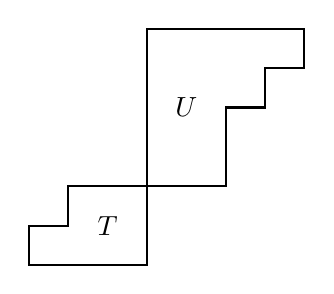
\begin{tikzpicture}[scale=.5, thick]
        \draw (0, 0) -- (2, 0) -- (2, 2) -- (3, 2) -- (3, 3) -- (4, 3) -- (4, 4) -- (0, 4) -- cycle;
        \draw (0, 0) -- (-2, 0) -- (-2, -1) -- (-3, -1) -- (-3, -2) -- (0, -2) -- cycle;
        \node at (1, 2) {\(U\)};
        \node at (-1, -1) {\(T\)};
    \end{tikzpicture}
    }}.
\end{equation}

\begin{lemma}
    Given tableaux \(T\) and \(U\),
    \begin{equation}
        \rowword(T \star U) = \rowword(T) \rowword(U) \equiv \rowword(T \leftarrow \rowword(U)).
    \end{equation}
\end{lemma}

Let \(a = a_1a_2 \dots a_r\) be a word.
Let \(L(a, 1)\) be the length of the longest weakly increasing subsequence of \(a\),
i.e., the largest \(k\) such that there exists a subsequence \(i_1 < i_2 < \cdots < i_k\) of \(\interval{r}\) such that \(a_{i_1} \leq a_{i_2} \leq \cdots \leq a_{i_k}\).

In general, let \(L(a, m)\) be the largest sum of the lengths of \(m\) disjoint weakly increasing subsequences of \(a\).

\begin{lemma}
    Let \(T \in \SSYT(\lambda)\).
    Then,
    \begin{equation}
        L(\rowword(T), m) = \lambda_1 + \lambda_2 + \cdots + \lambda_m.
    \end{equation}
\end{lemma}

\begin{proof}[Sketch]
    An increasing sequence of \(\rowword(T)\) uses at most one entry from each column of \(T\), and hence upper bound is achieved.
    Lower bound is achieved by taking the first \(m\) rows of \(T\).
\end{proof}

\begin{lemma}
    If \(w \equiv w'\), then \(L(w, m) = L(w', m)\) for all \(m\).
\end{lemma}

\begin{proof}[Sketch]
    It suffices to show that the existence of a collection of \(m\) disjoint weakly increasing subsequences of \(w\) with length sum \(\ell\) implies the existence of a collection of \(m\) disjoint weakly increasing subsequences of \(w'\) with length sum \(\ell\), when \(w \sim w'\) by elementary Knuth relations.

    Assume \(w = \mathbf{u} xzy \mathbf{v}\) and \(w' = \mathbf{u} zxy \mathbf{v}\).
    Let \(\mathcal{A}\) be a set of disjoint weakly increasing subsequences of \(w\) with length sum \(\ell\).
    If \(x\) and \(z\) are not in the same subsequence, then the same subsequences work for \(w'\) and we are done.
    Assume \(x\) and \(z\) are in the same subsequence, say \(\mathbf{a} \in \mathcal{A}\).
    If \(y\) is not used in any subsequence, then swap \(xz\) in \(\mathbf{a} \in \mathcal{A}\) for \(xy\) and we are done.
    If \(y\) is used in some subsequence \(\mathbf{b} \in \mathcal{A}\), we have \(\mathbf{a} \neq \mathbf{b}\).
    Write
    \begin{equation}
        \mathbf{a} = \mathbf{a}^{\leftarrow} xz \mathbf{a}^{\rightarrow}
        \qquad \text{and} \qquad
        \mathbf{b} = \mathbf{b}^{\leftarrow} y \mathbf{b}^{\rightarrow}.
    \end{equation}
    We change them to
    \begin{equation}
        \mathbf{a}^{\leftarrow} xy \mathbf{b}^{\rightarrow}
        \qquad \text{and} \qquad
        \mathbf{b}^{\leftarrow} z \mathbf{a}^{\rightarrow},
    \end{equation}
    and we are done.
    The other elementary Knuth relation is similar.
\end{proof}

\begin{theorem}
    Let \(w\) be a word.
    Then, the insertion tableau \(P(w)\) has shape \(\lambda = \composition{\lambda_1, \lambda_2, \ldots}\) where
    \begin{equation}
        \lambda_m = L(w, m) - L(w, m-1).
    \end{equation}
\end{theorem}

Let \(\tilde{L}(w, m)\) be the largest sum of the lengths of \(m\) disjoint strictly decreasing.
By repeating the same arguments and swapping the mentions of ``row'' and ``column'',
and ``weakly increasing'' and ``strictly decreasing'',
we obtain the following theorem.

\begin{theorem}
    Let \(w\) be a word.
    Then, the insertion tableau \(P(w)\) has shape \(\lambda = \composition{\lambda_1, \lambda_2, \ldots}\) where
    \begin{equation}
        \tilde{\lambda}_m = \tilde{L}(w, m) - \tilde{L}(w, m-1).
    \end{equation}
\end{theorem}

\begin{lemma}
    If \(w \equiv w'\) and an interval \(I \subset \positives\),
    then the subword of \(w\) obtained by taking the entries of \(w\) in \(I\) is plactically equivalent to the subword of \(w'\) obtained by taking the entries of \(w'\) in \(I\).
\end{lemma}

\begin{proof}[Sketch]
    The key is that, in a elementary Knuth relation,
    whenever \(x\) and \(z\) are in \(I\), then \(y\) is also in \(I\).
    Checking cases yields the result.
\end{proof}

\begin{theorem}
    For all words \(w\), there exists a unique \(T\) such that \(\rowword(T) \equiv w\).
\end{theorem}

\begin{proof}[Proof (existence)]
    The existence is immediate from RSK, since \(w \equiv \rowword(P(w))\).
\end{proof}

\begin{proof}[Proof (uniqueness)]
    It suffices to prove that, if \(T\) and \(U\) are tableaux such that \(\rowword(T) \equiv \rowword(U)\), then \(T = U\).
    We prove this by induction on the largest entry of \(T\) and \(U\), say \(M\).
    By previous lemmas, we have that \(\operatorname{sh}(T) = \operatorname{sh}(U)\).

    By deleting all instances of \(M\) from \(T\) and \(U\), we obtain tableaux \(T'\) and \(U'\) such that \(\rowword(T') = \left. \rowword(T) \right|_{\interval{M-1}} \equiv \left. \rowword(U) \right|_{\interval{M-1}} = \rowword(U')\).
    By induction, we have \(T' = U'\).
    Therefore, the boxes of \(T\) and \(U\) containing \(M\) are the entries in \(\operatorname{sh}(T) / \operatorname{sh}(T')\) and \(\operatorname{sh}(U) / \operatorname{sh}(U')\), respectively, which we know are the same.
    Therefore, \(T = U\).
\end{proof}

\begin{theorem}
    Let \(w\) be a word.
    The word \(w\) satisfies the backwards-Yamanouchi condition
    if and only if
    \(w \equiv \rowword(Y_\lambda)\) for some partition \(\lambda\),
    where \(Y_\lambda\) is the Yamanouchi tableau of shape \(\lambda\).
\end{theorem}

\begin{proof}
    First, we check that backwards-Yamanouchi is preserved by elementary Knuth relations.
    Since every word is plactically equivalent to a word of the form \(\rowword(T)\),
    and the only tableaux \(T\) that satisfy \(\rowword(T)\) is reverse Yamanouchi are the Yamanouchi tableaux,
\end{proof}

With this theorem, Littlewood--Richardson can be phrased as counting skew tableaux
whose reading words insert to a Yamanouchi tableau.